\documentclass[12pt]{article}

\usepackage[fleqn]{amsmath}
\usepackage{amssymb}
\usepackage{amsthm}
\usepackage{graphicx}
\usepackage{float}
\theoremstyle{plain}     %------- 'regular' theorem types
\newtheorem{thm}{Theorem}[section]
\newtheorem{cor}[thm]{Corollary}
\newtheorem{lemma}[thm]{Lemma}
\newtheorem{prop}[thm]{Proposition}
\newtheorem{example}[thm]{Example}
\newtheorem{exer}[thm]{Exercise}
\newtheorem{define}[thm]{Definition}
\usepackage[top=2cm, left=2cm, right=2cm]{geometry} 
\usepackage{parskip}
\setlength{\parindent}{0in}
\usepackage{floatflt}
\usepackage{multicol}
\usepackage{tabu}
\usepackage[hidelinks]{hyperref}
\hypersetup{
	urlcolor=blue}
\usepackage{enumitem}
%%%%%%%%%%%%%%%%%%%%%%
%%%%%%%%%%%%%%%%%%%%%%%
%%%%%%%%%%%%%%%%%%%%%%%%
\begin{document}
\large
%subject
City Semester  \hspace{8cm} Name:\makebox[6cm]{\hrulefill}
\\
%specific topic
A little quiz\\
\normalsize 
\emph{Complete all work on a separate sheet of paper with exercises clearly labeled and all reasoning and work given.}\\[.5cm]
%\emph{Show all work for full credit.}
\begin{enumerate}
	\item The following three equations model the populations for three different towns a, b, and c in years:
		\begin{enumerate}[label=(\roman*)]
			\item $P_a(t)=1000(1.12)^t$\\
			\item $P_b(t)=2500(.8)^t$\\
			\item $P_c(t)=500(2)^2$\\
		\end{enumerate}
		\begin{enumerate}
			\item Which towns have growing populations? Which have shrinking populations?
			\item Which town is growing the fastest? What is its annual percent growth?
			\item What is the population of town b after 10 years?
		\end{enumerate}
	

	\item An exponential function of the form $y=ab^x$ passes through the points $\left(-2,400\right)$ and $\left(2,\dfrac{2}{5}\right)$. Find the equation of this exponential.
	\item Explain how to distinguish a linear function from an exponential function.
	\item (anyone can try it, but this is required for intensive). Note: $t_0$ is the x-coordinate of the point where the two exponentials meet.\\
	\begin{figure}[H]
		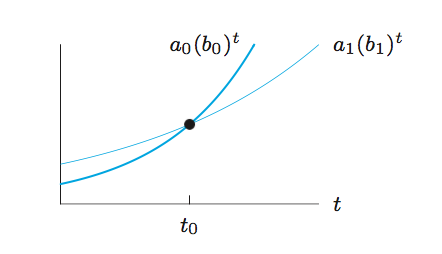
\includegraphics[scale=.5]{1.png}
	\end{figure}
		\begin{enumerate}
			\item What happens to $t_0$ if $a_0$ is increased while $a_1$, $b_1$ and $b_0$ remain fixed?
			\item What happens to $t_0$ if $b_1$ is decreased while $a_1$, $b_0$ and $a_0$ remain fixed?
		\end{enumerate}

\end{enumerate}
	
\end{document} 